\section*{Dati e risultati}

\subsection*{Raddrizzatore di precisione a semionda}

\begin{wrapfloat}{figure}{O}{0pt}
        \def\svgwidth{0.45\textwidth}
        \subimport{figure/}{raddrizzatore.pdf_tex}
        \caption{Raddrizzatore di precisione a semionda. Alimentato, inizialmente con una $V\ped{in}\,=\,\SI{1.02}{\volt}$ di frequenza $\nu\,=\,\SI{50}{\hertz}$.}
        \label{fig:radd}
\end{wrapfloat}

Lo scopo di questo raddrizzatore di precisione a semionda è lo stesso di quello di un normale raddrizzatore di tensione asemionda. Tuttavia vi è una caratteristica sostanzialmente differente tra le due tiplogie di raddrizzatori di tensione. Nel caso di un raddrizzatore normale, quindi di un circuito che sfrutta solo le peculiarità di un diodo, vi è una differenza di potenziale ai capi del diodo (normalmente, se il diodo è al silicio, questa ddp. vale $\SI{0.6}{\volt}$). Questa differenza di potenziale si riperquote sul segnale in uscita ($V\ped{out}$), che pur seguendo fedelmente il segnale in ingresso ($V\ped{in}$) risulterà attenuato di $\SI{0.6}{\volt}$ rispetto a $V\ped{in}$.
Invece per quanto riguarda il raddrizzatore di precisione, grazie alla sua configurazione, Figura \ref{fig:radd}, permette di non avere sul segnale in uscita la caduta di tensione in diretta del diodo, e quindi di seguire ancora più fedelmente il segnale in ingresso al circuto.
Naturalmente tutta la parte di segnale in ingresso negativa non viene minimamante presa in considerazione dal momento che il diodo, in entrambe le configurazioni, risulterebbe interdetto, quindi non vi è passaggio di corrente. Infatti per tutto il tempo in cui il segnale in ingresso è negativo l'amplificatore si trova in saturazione negativa e quindi $V\ped{ol}\,=\,V\ped{cc}^-$. Con $V\ped{cc}^-$ indichiamo il valore di saturazione negativa dell'amplificatore operazionale.

Ora passiamo ad un'analisi più approfondita del nostro circuito (Figura \ref{fig:radd}). Come possimo subito notare l'amplificatore operazionale è in configurazione emitter follower non invertente. Quindi in prima approssimazione si ha che $V\ped{in}\,\equiv\,V\ped{out}$. Ora dal momento che in uscita vi è un diodo verrebbe naturale pensare che il segnale in uscita debba essere attenuato di $\SI{0.6}{\volt}$ rispetto a quello in ingresso. Questo non accade per il seguente motivo, che possiamo comprendere grazie all'analisi circuitale del sistema. Grazie alle regole per gli amplificatori operazionali abbiamo quanto segue:
\begin{equation}
        \left\{
                \begin{array}{l l}
                        V\ped{ol}\,=\,A(V^+ - V^-)\\
                        V\ped{out}\,=\,V\ped{ol}-\Delta V
                \end{array}
         \right.
         \label{eq:radd_1}
\end{equation}
dove con $V\ped{ol}$ abbiamo indicato la differenza di potenziale all'anodo del diodo, con $\Delta V$ indichiamo la caduta in diretta del diovo che vale circa $\SI{0.6}{\volt}$ ed A simboleggia l'amplificazione del nostro amplificatore operazionale.
A questo punto osserviamo che sussistono le seguenti relazioni: $v^+\,=\,V\ped{in}$ e $V^-\,=\,V\ped{out}$. Pertanto grazie a dei semplici passaggi algebrici possiamo ottenere che:
\begin{equation}
        V\ped{in}\,=\,\left(1+\frac{1}{A}\right)V\ped{out} + \frac{\Delta V}{A}
\end{equation}
Quindi se teniamo conto del fatto che per un amplificatore operazonale UA741 il valore di A è circa $10^5$ possiamo concludere che il termine $\frac{\Delta V}{A}$ è trascurabile in quanto si otterrebbe una differenza di potenziale di circa $\SI{6}{\micro\volt}$, irrilevante se paragonata al segnale in ingresso che è dell'ordine del $\si{\volt}$. Inoltre sempre per l'elevato valore di A possiamo porre anche $\left(1+\frac{1}{A}\right)\,\simeq\,1$. Quindi l'equazione (\ref{eq:radd_1}) si può approssimare come segue:
\begin{equation}
        V\ped{in}\,\simeq\,V\ped{out}
        \label{eq:radd_2}
\end{equation}
che rappresenta il risultato atteso, ovvero che l'output del circuito riproduce fedelmente la parte positiva del segnale in ingresso.
Questi risultati si possono osservare anche andando ad analizzare il grafico in Figura \ref{fig:radd_plot1}

Nei grafici in Figura \ref{fig:radd_plot1} si può chiaramente osservare che per quanto riguarda il comportamento del segnale di output ($V\ped{out}$) in funzione di $V\ped{in}$ tutto funziona correttamente, come da previsioni teoriche. Questo è valido anche se osserviamo l'andamento di $V\ped{ol}$ in funzione di $V\ped{in}$. In questo caso possiamo osservare come, per la parte di $V\ped{in}$ positiva $V\ped{ol}$ ne segua correttamente l'andamento, mentre quando $V\ped{in}$ diventa negativo $V\ped{ol}$ assume quasi istantaneamente il valore di saturazone negativa $V\ped{cc}^-$.

Come è possibile notare dal grafico riportato in Figura \ref{fig:radd_plot2}, vi è un ritardo da parte dell'amplificatore nel seguire, in salita, il segnale in ingresso. Questo ritardo come abbiamo pensato inizialmente non è dovuto allo slew rate dell'amplificatore, anche se in minima parte contribuisce, bensì ad un problema di progettazione del circuito.
Ovvero, nel momento in cui il segnale in ingresso assume valori negativi la tensione $V\ped{ol}$ si trova in saturazione negativa, il diodo è interdetto quindi $V\ped{out}$ che ha lo stesso alore di $V^-$ (causa retroazione negativa), si trova ad una differenza di potenziale nulla. Quindi quando il seganle in ingresso diventa positivo l'amplificatore impiega del tempo prima di portare tutti i suoi componenti interni dalla regione di saturazione negativa ad un regime positivo. Questo lasso di tempo si può identificare pertanto con il ritardo visibile in Figura \ref{fig:radd_plot2}. Inoltre abbiamo notato che aumentando la frequenza del segnale in ingresso il tempo di risposta dell'amplificatore diminuisce. Questo molto probabilmente è dovuto al fatto che sempre meno componenti interni dell'amplifictore si portano completamente in $V\ped{cc}^-$.
Per concludere e dare maggior validità a queste ipotesi possiamo dire che questo ritardo non si accusa quando $V\ped{in}$ passa da positivo a negativo. In questo caso infatti $V\ped{ol}$ può seguire l'andamento del segnale in ingresso in quanto non deve fare fronte ad un improvvisa e importante differenza di potenziale come durante la fase di salita. 
Per oviare a questo problema si possono apportare alcune modifiche al circuto che andremo a discutere nel paragrafo seguente.

\subsection*{Raddrizzatore di precisione a semionda ottimizzato}

\begin{wrapfloat}{figure}{I}{0pt}
        \def\svgwidth{0.5\textwidth}
        \subimport{figure/}{radd_ott.pdf_tex}
        \caption{Raddrizzatore di precisione a semionda ottimizzato.}
        \label{fig:radd_ott}
\end{wrapfloat}

In questa sezione ci occupiamo di discutere i vantaggi di un raddrizzatore a semionda realizzato come in Figura \ref{fig:radd_ott}. Come accennato nel paragrafo precedente il grande problema della configurazione precedente è quello che per $V\ped{in}$ negativi $V\ped{ol}$ raggiungeva quasi istantaneamente il valore di tensione tensione $V\ped{cc}^-$ e quindi in salita vi era un lasso temporale in cui $V\ped{out}$ manteneva un valore di tensione nullo a dispetto di un $V\ped{in}$ in ingresso positivo (Figura \ref{radd_plot2}).

Per ovviare a questo inconveniente abbiamo realizzato il circuito illustrato in Figura \ref{fig:radd_ott}. La parte fondamentale risiede nell'inserimento di un secondo diodo (D2) e delle due resistenze $R_1$ e $R_2$.

Passiamo ora ad una discussione sull'andamento del segnale in uscita $V\ped{out}$ in funzione di $V\ped{in}$. Quando $V\ped{in}$ è positivo abbiamo che il segnae di output risulta esser, con le approssimazioni discusse anche nel paragrafo precedente:
\begin{equation}
        V\ped{out}\,=\,-V\ped{in}\,\frac{R_2}{R_1}
\end{equation}
e dal momento che $R_1\,=\,R_2$ il segnale in uscita è una replica del segnale in ingresso sfasato di $\pi$.
Tuttavia NON HO PIU' VOGLIA. 

SCUSA PASA DOMANI LA FINISCO PERDONAMI CHIEDO VENIA, QUESTA MATTINA È STATA UN INFERNO!!!!!!!!!!























































%\begin{wrapfloat}{figure}{O}{0pt}
%        \def\svgwidth{0.45\textwidth}
%        \subimport{figure/}{comparatore.pdf_tex}
%        \caption{Circuito realizzato per lo studio delle proprietà del comparatore. Il comparatore utilizzato è l'LM311.}
%        \label{fig:comparatore}
%\end{wrapfloat}

%\begin{SCfigure}
%    \centering
%    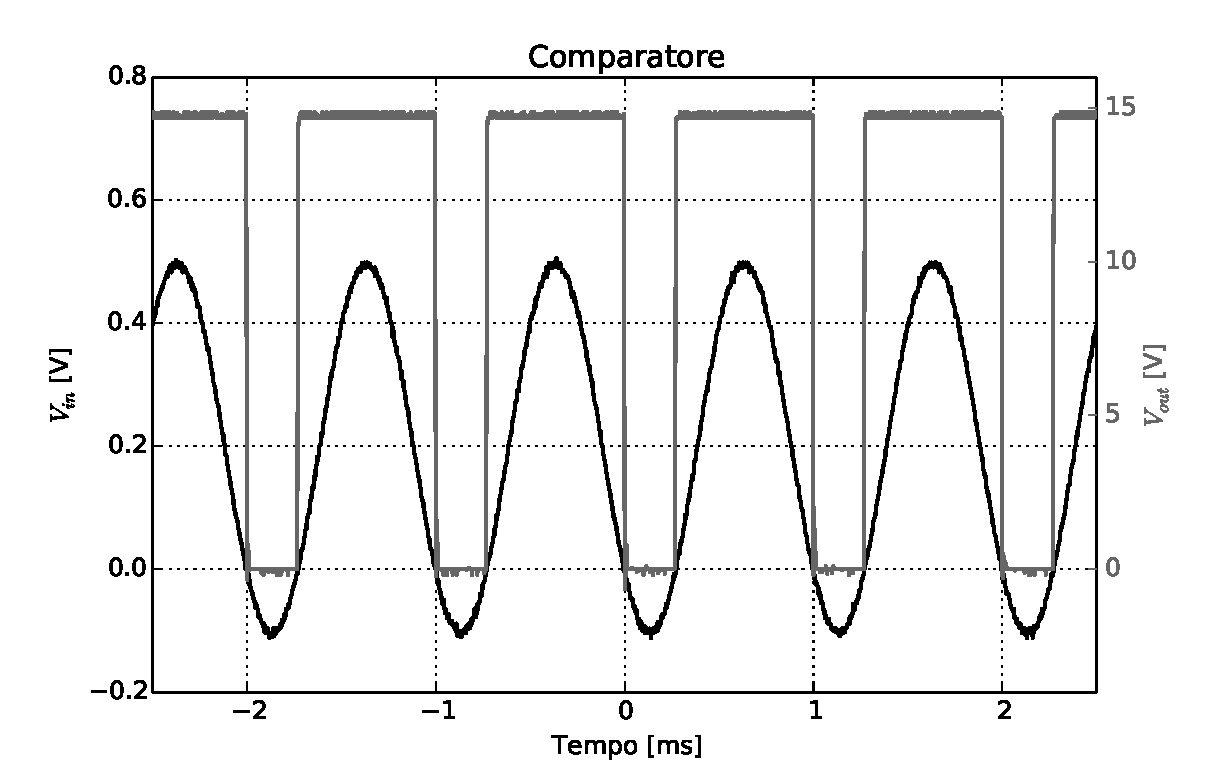
\includegraphics[width=0.75\textwidth]{figure/comp_graph.pdf}
%    \caption{Il grafico mostra l'andamento del segnale in ustita ($V\ped{out}$), onda quadra, dal nostro comparatore LM311 fornito un segnale in ingresso sinusoidale. Come è possibile notare il segnale in uscita $V\ped{out}$ assume il valore di saturazione positiva $V\ped{sat}^+\,=\,\SI{}{\volt}$ ogni volta che $V\ped{in}\,\geq\,\SI{0}{\volt}$, mentre $V\ped{out}\,=\,\SI{0}{\volt}$ quando $V\ped{in}\,\leq\,\SI{0}{\volt}$. Inoltre è possibile osservare che il segnale in ingresso ha un offset di $\SI{0.2}{\volt}$.}
%    \label{fig:comparatore_plot}
%\end{SCfigure}

%\begin{figure}[H]
%    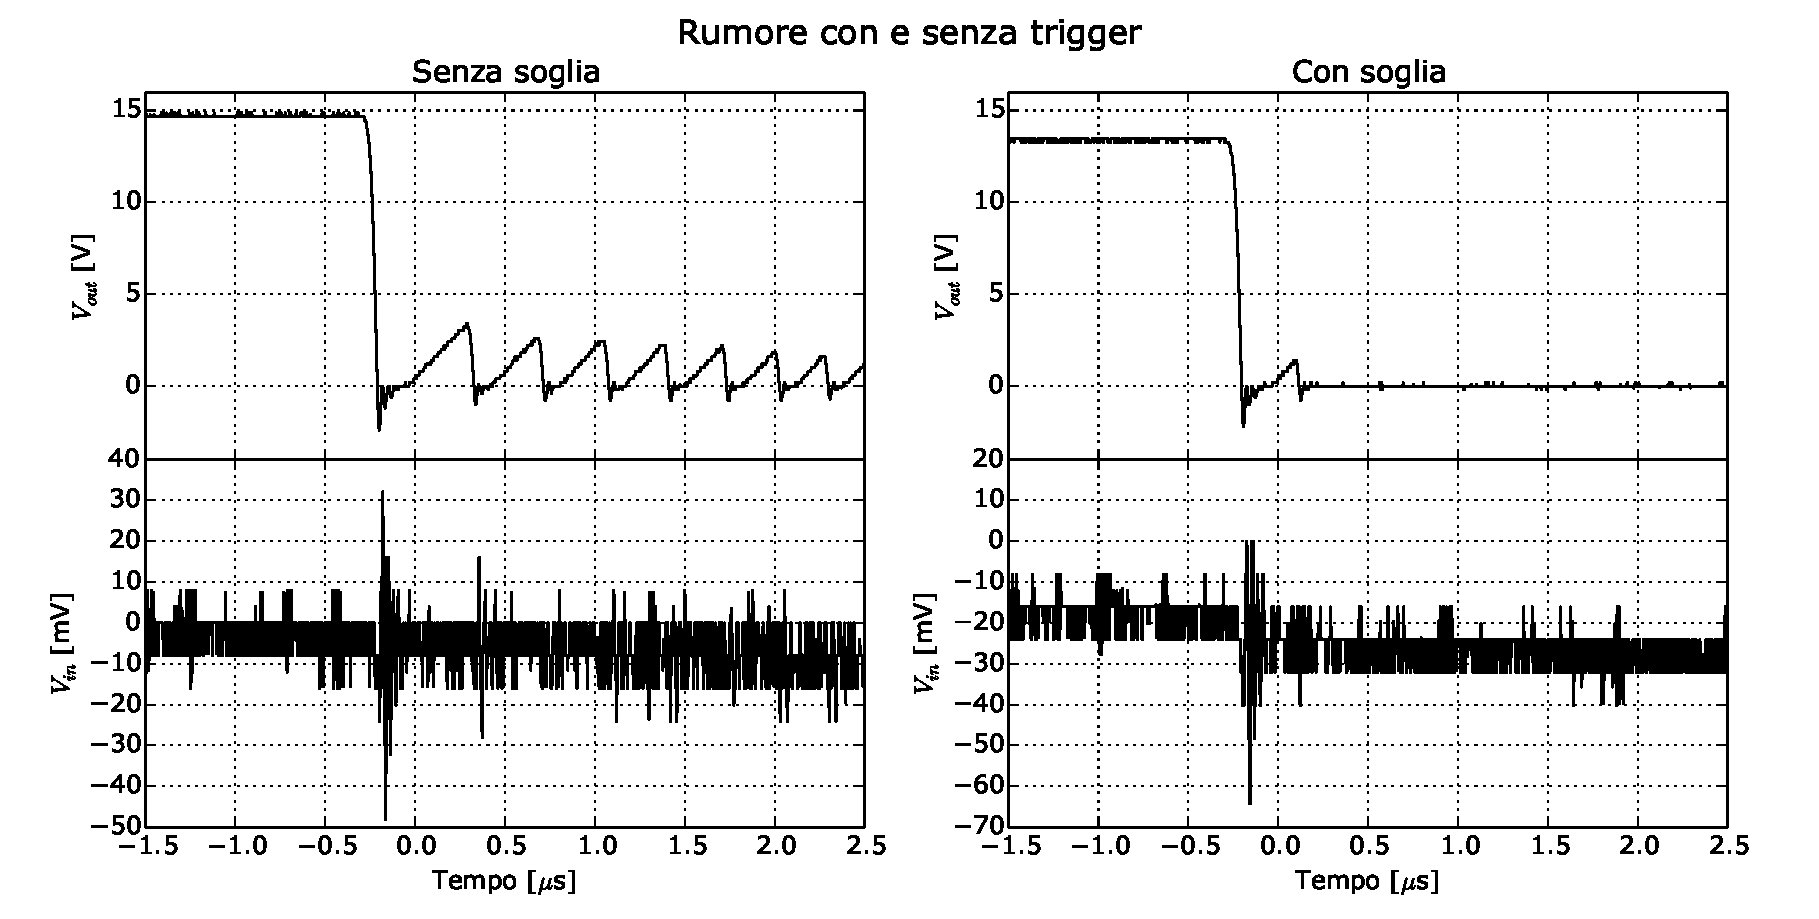
\includegraphics[width=\textwidth]{figure/trigger_graph.pdf}
%    \caption{Questa immagine mostra un paragone tra il risultato che si otterrebbe con un comparatore senza trigger di Schmitt, nella figura a sinistra, e un comparatore dotato di questo trigger, figura a destra. Come si può chiaramente osservare nel caso in cui il comparatore sia dotato di trigger gli effetti del rumore sul segnale in uscita sono molto meno visibili. Questo è merito della doppia soglia che permette di non far scattare il comparatore appena il segnale in ingresso assume valore positivo o negativo, ma come già spiegato, ammette un range di tensioni, che sono un intorno dello zero, per le quali il segnale in output mantiene il suo valore, positivo o negativo che fosse. Il nostro intervallo di accettazione è:$V\ped{OL}\,=\,(-12.9\pm0.1)\SI{}{\milli\volt}$, soglia bassa e $V\ped{OH}\,=\,\SI{0}{\milli\volt}$, soglia alta.}
%    \label{fig:schmitt_plot}
%\end{figure}


